% Generated from arXiv:2503.18741; see tools/build_source_compendium.py.
\section{Calculation laboratory III: From a Stokes graph to a resonance width}
\label{lab:2503_18741}

\calculationroute
  {Asymptotic scattering coefficients, the Riccati recursion, lateral Borel sums, simple-turning-point connection matrices, and the no-incoming-wave condition.}
  {Scattering poles, the cubic oscillator, and the complete inverted Rosen--Morse calculation, including its repeated Stokes geometry.}
  {Reproduce the inverted Rosen--Morse pole condition and decay width from the ordered Stokes data and verify them against the exact solution.}

This Laboratory reconstructs the calculation underlying
Ref.~\cite{Morikawa:2025grx}.  Scattering and exact-WKB definitions have
already been fixed in Stages II and III; the source-paper recapitulation is
therefore omitted.  What follows is the model-specific Stokes transport,
including the original intermediate algebra and TikZ geometry.

\begin{comment}
\subsection{Resonant states in scattering theory}\label{src:2503_18741:sec:resonance}
Figure~\ref{src:2503_18741:fig:pole-a} shows that bound and resonant states appear as poles of an S-matrix and are characterized by the complex wave number~\cite{Taylor:1972}. 
Resonances exist in the fourth quadrant of the complex $k$-plane.
Bound states are distributed along the negative region of the real axis in the complex $E$-plane, while resonant states are in the fourth quadrant as shown in Fig.~\ref{src:2503_18741:fig:pole-b}.
\begin{figure}[t]
 \centering
 \begin{subfigure}{0.45\columnwidth}
  \centering
  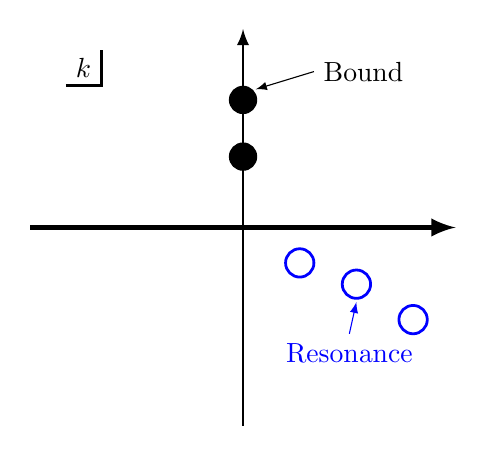
\begin{tikzpicture}[x=0.9mm,y=0.9mm,>=latex]
   %axis
   \draw[->,line width=2pt] (-30,0) -- (30,0);
   \draw[->,line width=1pt] (0,-28) -- (0,28);
   %k
   \draw[line width=1pt] (-25,20) -- (-20,20) -- (-20,25);
   \draw[line width=1pt] (-22.5,22.5) node {$k$};
   %circle white
   \draw[line width=1pt,blue] (8,-5) circle (2);
   \draw[line width=1pt,blue] (16,-8) circle (2);
   \draw[line width=1pt,blue] (24,-13) circle (2);
   %cross
   %\draw[line width=1pt] (-10+1/1.4,-3-1/1.4) -- (-6-1/1.4,-7+1/1.4);
   %\draw[line width=1pt] (-10+1/1.4,-7+1/1.4) -- (-6-1/1.4,-3-1/1.4);
   %\draw[line width=1pt] (-18+1/1.4,-6-1/1.4) -- (-14-1/1.4,-10+1/1.4);
   %\draw[line width=1pt] (-18+1/1.4,-10+1/1.4) -- (-14-1/1.4,-6-1/1.4);
   %\draw[line width=1pt] (-26+1/1.4,-11-1/1.4) -- (-22-1/1.4,-15+1/1.4);
   %\draw[line width=1pt] (-26+1/1.4,-15+1/1.4) -- (-22-1/1.4,-11-1/1.4);
   %circle black
   \fill (0,10) circle (2);
   \fill (0,18) circle (2);
   %description
   \draw[<-] (1.8,19.5) -- (10,22) node[right] {Bound};
   \draw[<-,blue] (16,-10.5) -- (15,-15) node[below] {Resonance};
   %\draw[<-] (-16,-10.5) -- (-22,-15) node[below] {Anti-Resonance};
  \end{tikzpicture}
  \caption{Complex $k$-plane}
  \label{src:2503_18741:fig:pole-a}
 \end{subfigure}
 \begin{subfigure}{0.45\columnwidth}
  \centering
  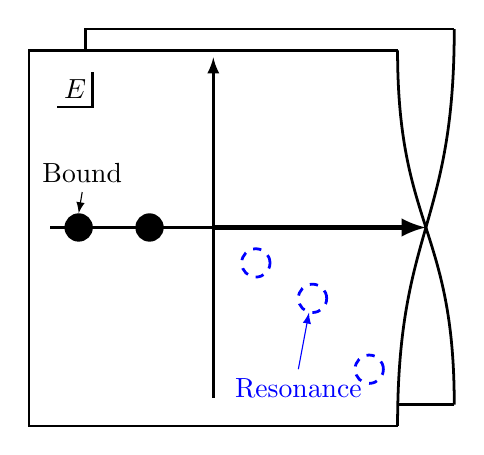
\begin{tikzpicture}[x=0.9mm,y=0.9mm,>=latex]
   %Riemann
   \draw[line width=1pt] (22,25) .. controls (22,0) and (30,0) .. (30,-25);
   \draw[line width=1pt] (30,28) .. controls (30,0) and (22,0) .. (22,-28);
   \draw[line width=1pt] (22,25) -- (-30,25) -- (-30,-28) -- (22,-28);
   \draw[line width=1pt] (30,28) -- (-22,28) -- (-22,25);
   \draw[line width=1pt] (30,-25) -- (22,-25);
   %axis
   \draw[line width=1pt] (-27,0) -- (-4,0);
   \draw[->,line width=2pt] (-4,0) -- (26,0);
   \draw[->,line width=1pt] (-4,-24) -- (-4,24);
   %E
   \draw[line width=1pt] (-26,17) -- (-21,17) -- (-21,22);
   \draw[line width=1pt] (-23.5,19.5) node {$E$};
   %circle white
   \draw[blue,dashed,line width=1pt] (2,-5) circle (2);
   \draw[blue,dashed,line width=1pt] (10,-10) circle (2);
   \draw[blue,dashed,line width=1pt] (18,-20) circle (2);
   %cross
   %\draw[black!60,line width=1pt] (1/1.4,3+1/1.4) -- (4-1/1.4,7-1/1.4);
   %\draw[black!60,line width=1pt] (1/1.4,7-1/1.4) -- (4-1/1.4,3+1/1.4);
   %\draw[black!60,line width=1pt] (8+1/1.4,8+1/1.4) -- (12-1/1.4,12-1/1.4);
   %\draw[black!60,line width=1pt] (8+1/1.4,12-1/1.4) -- (12-1/1.4,8+1/1.4);
   %\draw[black!60,line width=1pt] (16+1/1.4,18+1/1.4) -- (20-1/1.4,22-1/1.4);
   %\draw[black!60,line width=1pt] (16+1/1.4,22-1/1.4) -- (20-1/1.4,18+1/1.4);
   %circle black
   \fill (-13,0) circle (2);
   \fill (-23,0) circle (2);
   %description
   \draw[<-] (-23,2) -- (-22.5,5) node[above] {Bound};
   \draw[blue,<-] (9.5,-12) -- (8,-20) node[below] {Resonance};
   %\draw[black!60,<-] (8,12) -- (-3,17) node[above] {Anti-Resonance};
  \end{tikzpicture}
  \caption{Complex $E$-plane}
  \label{src:2503_18741:fig:pole-b}
 \end{subfigure} 
 \caption
 {Distribution of S-matrix poles in (a) the complex $k$-plane and (b) the complex $E$-plane. In the right panel~(b), the bound states exist in the first Riemann surface, while the resonant states appear in the second Riemann surface.}
 \label{src:2503_18741:fig:pole}
\end{figure}
Note that bound and resonant states exist in the first and second Riemann surfaces, respectively, of the complex $E$-plane. A resonant state has complex energy, where the real part is the resonant energy and the imaginary part is the decay width. Resonance is produced by the scattering of multiple particles. If the decay width is narrow, a resonant state is observed as a sharp peak in the energy spectrum of the cross-section. 
The singular nature of a resonant state, which is the divergence of the wave function in the asymptotic region, causes difficulty in investigating the state. In the $3$D space, the radial wave function $\varphi(r)$ of a resonant state with $k=k_{r}-\rmi k_{i}$ ($k_{r}$, $k_{i}\in\mathbb{R}^{+}$) has the following asymptotic form:
\begin{align}
 \varphi(r) \xrightarrow[r\to\infty]{}\rme^{\rmi kr} = \rme^{\rmi k_{r}}\rme^{k_{i}r},
\end{align}
which diverges due to the factor $\rme^{k_{i}r}$. This property also leads to the divergence of the norm, $||\varphi(r)||^2$. To obtain a finite value of the norm, the Zel'dovich regularization~\cite{Zel'dovich:1961} is introduced as
\begin{align}
 ||\varphi(r)||^2\equiv\lim_{\varepsilon\to+0}\int_{0}^{\infty} \rmd r\, \rme^{-\varepsilon r^2}\varphi(r)^2r^2 .
\end{align}
Using this regularization, the orthogonality and completeness properties of the resonant states have been proved by Berggren~\cite{Berggren:1968zz}. It should be noted that the square of the wave function is integrated with the norm of the resonant state.
Recently, the CSM~\cite{Aguilar:1971ve,Balslev:1971vb,Myo:2014ypa} has been developed as another way to overcome the divergence of the norm and has been applied to describe resonant states of many-body systems, such as nuclei, atoms, and molecules. In the CSM, the coordinate $r$ is transformed as $r\to \rme^{\rmi \theta}r$ with a parameter $\theta$. The ABC theorem argues that resonance, which is obtained from a Hamiltonian with this transformation, is square integrable. This can be naively understood as follows: In the CSM, the asymptotic form of the resonant wave function is transformed as
\begin{align}
 \rme^{\rmi kr} \rightarrow \rme^{\rmi (k_{r}-\rmi k_{i})re^{\rmi \theta}}=\rme^{(-k_{r}\sin\theta+k_{i}\cos\theta)r}\rme^{\rmi (k_{r}\cos\theta+k_{i}\sin\theta)r},
\end{align}
which converges when $\theta>\tan^{-1}(k_{i}/k_{r})$.
The CSM thus enables a square-integrable treatment of resonant states by rotating the coordinate into the complex plane and has been successfully applied to many-body systems. Complementary approaches, such as the Gamov shell model~\cite{Michel:2009}, have also been developed to tackle the divergence problem inherent in resonant states.
\subsection{Exact WKB analysis and decay rate}\label{src:2503_18741:sec:ewkb}
\subsubsection{Brief introduction of exact WKB analysis}
The $1$D Schr\"odinger equation can be written as
\begin{align}
    \left[-\frac{\hbar^2}{2}\frac{\rmd^2}{\rmd x^2}+V(x)\right] \psi(x)
    = E \psi(x) .
\end{align}
For simplicity, we set
\begin{align}
    \left[-\frac{\rmd^2}{\rmd x^2}+\hbar^{-2}Q(x)\right] \psi(x) = 0,
    \qquad Q(x) = 2\left[V(x)-E\right] .
\end{align}
The WKB solution is an ansatz defined by a formal power series,
\begin{align}
    \psi(x,\hbar) &= \rme^{\int^x \rmd x'\, S(x',\hbar)} ,&
    S(x,\hbar) &= \sum_{i=-1}^{\infty}\hbar^{i} S_{i}(x) .
\end{align}
Substituting $S(x,\hbar)$ into the Schr\"odinger equation,
we have the nonlinear Riccati equation;
we can obtain the recursive equation of $S_i$.
The leading order of the recursive equation is given by
\begin{align}
    S_{-1}(x) = S_{-1}^{\pm}(x) \equiv \pm \sqrt{Q(x)} .
\end{align}
It is known that (i) $S_i^{-}=(-1)^i S_i^{+}$,
(ii) $S^{\pm}=\pm \vsub{S}{odd} + \vsub{S}{even}$,
where $\vsub{S}{odd}=\sum_{i=-1,1,3,\dots}\hbar^i S_i^{+}$
and $\vsub{S}{even}=\sum_{i=0,2,4,\dots}\hbar^i S_i$,
(iii) $\vsub{S}{even}=-\frac{1}{2}\frac{\rmd}{\rmd x}\ln \vsub{S}{odd}$, and also (iv) the exact solution and approximation of the WKB wave function are
\begin{align}
    \psi(x,\hbar)^{\pm} = \frac{1}{\sqrt{\vsub{S}{odd}}}
    \rme^{\pm\int_{x_0}^x \rmd x'\, \vsub{S}{odd}} 
    \sim \frac{1}{Q^{1/4}} \rme^{\pm\hbar^{-1}\int_{x_0}^x \rmd x'\, \sqrt{Q}} + \dots.
\end{align}
The formal series is not necessarily convergent,
and one uses the so-called Borel resummation to give a finite value.
The essential point is the insertion of one,
\begin{align}
    1 = \frac{1}{\Gamma(n+\alpha)} \int_0^\infty \rmd x\, \rme^{-x} x^{n+\alpha-1},
\end{align}
and exchange of the infinite sum and the above integral.
Now, the infinite sum becomes a convergent series,
while the integral may be singular for some parameters,
called Borel singularity.
Then, because the total value is ill-defined,
we pick up some analytically continued paths
that have an imaginary and nonperturbative nontrivial difference.
When the path jumps over the Borel singularity,
such a function suddenly changes (Stokes phenomenon).
In the exact WKB analysis, we can see such a condition
in terms of~$Q$ as
\begin{align}
    \im \hbar^{-1} \int^x \rmd x' \sqrt{Q} = 0.
\end{align}
The curves determined by this condition are called Stokes curves,
and the structure is a Stokes graph.
\end{comment}
\subsection{Worked Stokes geometry: cubic decay and the solvable barrier}
The definitions of lateral Borel sum, Stokes curve, and connection matrix are
those of Sec.~\ref{sec:exact-wkb}.  We now apply them without redefining them.
\subsubsection{Application to unstable QM: Anharmonic oscillator with cubic potential}
As an example, let us consider the cubic potential, $V(x) = x^2(1-x)$.
This is not well-defined but is pedagogical for our purpose.
The Stokes graph for~$0<E<\max V(x>0)$ is shown in Fig.~\ref{src:2503_18741:fig:cubic}.
The black solid curves are the Stokes curves.
The index of each curve $\pm$ implies that $\psi^{\pm}$ increases exponentially and
\begin{align}
    \re \hbar^{-1} \int^x \rmd x' \sqrt{Q} \gtrless 0.
\end{align}
Three Stokes curves gather at one point, called the turning point, which is depicted as a black point.
The blue wavy lines are branch cuts.
\begin{figure}
    \centering
\begin{tikzpicture}
    \draw[thick] (2,0) -- (0,0) node[left] {$-$};
    \draw[thick] (2,0) .. controls (2.5,0.5) and (2.5,1).. (2.7,2) node[above] {$+$};
    \draw[thick] (2,0) .. controls (2.5,-0.5) and (2.5,-1).. (2.7,-2) node[below] {$+$};
    \draw[thick] (4,0) .. controls (3.5,0.5) and (3.5,1).. (3.3,2) node[above] {$+$};
    \draw[thick] (4,0) .. controls (3.5,-0.5) and (3.5,-1).. (3.3,-2) node[below] {$+$};
    \draw[thick] (4,0) -- (6,0) node[midway,below] {$-$};
    \draw[thick] (6,0) .. controls (6.5,0.5) and (6.5,1).. (6.7,2) node[above] {$+$};
    \draw[thick] (6,0) .. controls (6.5,-0.5) and (6.5,-1).. (6.7,-2) node[below] {$+$};
    %
    \draw[very thick,blue,snake it] (2,0) -- (4,0);
    \draw[very thick,blue,snake it] (6,0) -- (8,0);
    %
    \fill (2,0) circle(3pt) node[below left] {$a_1$};
    \fill (4,0) circle(3pt) node [below right] {$a_2$};
    \fill (6,0) circle(3pt);
    %
    \draw[very thick,red,->] (0,0.2) -- (6,0.2) .. controls (6.4,0.7) and (6.4,1.2).. (6.55,2);
    %
    \node at (1,1) {I};
    \node at (3,1) {II};
    \node at (5,1) {III};
\end{tikzpicture}
    \caption{Stokes graphs for the cubic potential.
    The black solid curves are the Stokes curves
    and black points are the turning points connecting three Stokes curves.
    The blue wavy lines are branch cuts.
    The red arrowed curve is a possible physical path on which the wave function is defined.}
    \label{src:2503_18741:fig:cubic}
\end{figure}
Due to the unbounded potential, it is difficult to define physical phenomena only on~$x\in(-\infty,\infty)$.
For example, let us choose the red arrowed path and then see what happens.
At first, near $x=-\infty$, $\psi^{-}$ sufficiently decreases and so is normalizable.
When we jump over the Stokes curve with the index~$+$ starting from the same turning point (I$\to$II), the Stokes phenomenon gives rise to
\begin{align}
    \begin{pmatrix}
      \vsub{\psi^{+}}{I} \\ \vsub{\psi^{-}}{I}
    \end{pmatrix}
    =
    M
    \begin{pmatrix}
      \vsub{\psi^{+}}{II} \\ \vsub{\psi^{-}}{II}
    \end{pmatrix} ,
    \label{src:2503_18741:eq:connection}
\end{align}
where $M$ depends on the rotation of the path around the turning point,
\begin{align}
    M =
    \begin{cases}
        M_{+} & \text{if anticlockwise for the index~$+$,} \\
        M_{+}^{-1}& \text{if clockwise for the index~$+$,} \\
        M_{-} & \text{if anticlockwise for the index~$-$,} \\
        M_{-}^{-1} &\text{if clockwise for the index~$-$,}
    \end{cases}
\end{align}
and
\begin{align}
    M_{+} &=
    \begin{pmatrix}
        1 & \rmi \\ 0 & 1
    \end{pmatrix}, &
    M_{-} &=
    \begin{pmatrix}
        1 & 0 \\ \rmi & 1
    \end{pmatrix} .
\end{align}
The above matrix is called the monodromy matrix.
Inside region II, we need to connect the different turning points, $a_1$ and $a_2$.
The wave function is related to each other by the factor,
\begin{align}
    \rme^{\pm\int_{a_1}^{a_2}\rmd x\, \vsub{S}{odd}}
\end{align}
Finally, in the exchange of regions II and III, we again use the connection rule~\eqref{src:2503_18741:eq:connection}.
If this system is just the harmonic oscillator, $V(x)=x^2$,
the above strategy completes our task.
For the wave function to converge near~$x=\infty$,
we have the quantization condition
\begin{align}
    1 + A = 0, \qquad
    A = \rme^{\oint \rmd x\, \vsub{S}{odd}} .
\end{align}
Here the cycle, $A$, comes from the connection between the turning points~$a_1$ and $a_2$.
Actually, by analytically continuing,
$A$ can be rewritten as the integral around the point of infinity.
That is, $A=\rme^{2\pi \rmi  \hbar^{-1} E}$;
we have the usual quantized energy spectrum~$E=\hbar\left(n+\frac{1}{2}\right)$ with $n\in\mathbb{Z}_{\geq0}$.
Now, for the cubic potential, the analytical continuation should be stuck because of the branch cut attached to the point of infinity.
However, a path on the upper-half plane must differ from that on the lower-half plane.
This reproduces the usual result of some kind of tunneling analysis.
This section is now finished but we will see a concrete result
being identical to the exact solution.
\subsection{Resonant states in exact WKB analysis}\label{src:2503_18741:sec:res_ewkb}
\subsubsection{What is a resonant state from the viewpoint of exact WKB?}\label{src:2503_18741:sec:view_res}
Given a potential $V(x)$ as a function of~$x\in\mathbb{R}$,
let us complexify the coordinate as $z\in\mathbb{C}$.
In the complex plane~$z$,
if the potential $\re V(z)$ possesses local minima, all of which are not stable physical states,
then the Hilbert space of the system includes resonant states.
This is because observations from the exact WKB analysis, i.e. structures of Stokes curves, are sensitive to the change of signs of~$V(z)-E$.
For instance, in an unusual harmonic oscillator, $V(x)=-x^2$,
one finds that in~Fig.~\ref{src:2503_18741:fig:V_harmonic} there is no local minimum; no resonant state exists.
On the other hand, some kind of potential has the local minimum which is not a true vacuum, such as in~$1/\cosh^2(x-a)+1/\cosh^2(x+a)$; there are resonant states.
Additionally, it is known that for the potential,
$V(x)=1/\cosh^2{x}$,
we observe nontrivial complex energies of resonance.
This is the so-called barrier resonance,
which traps the wave function into the bump.
In fact, in~Fig.~\ref{src:2503_18741:fig:V_cosh}, we can see the existence of local minima in $\re V(z)$ with~$\im z\neq0$.
\begin{figure}
    \centering
    \begin{subfigure}{0.48\columnwidth}
        \centering
        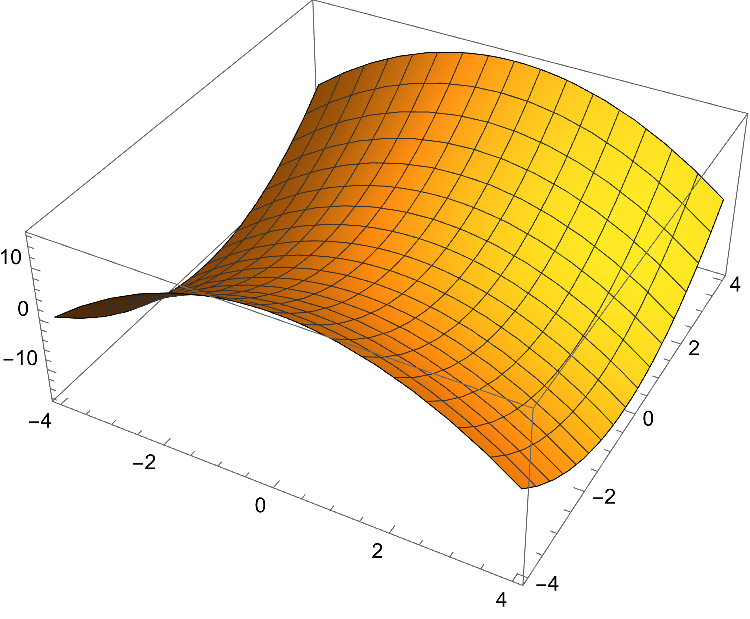
\includegraphics[width=\columnwidth]{source_compendium/figures/2503_18741/fig/harmonic_re.pdf}
        \caption{Real part}
    \end{subfigure}\hspace*{1em}
    \begin{subfigure}{0.48\columnwidth}
        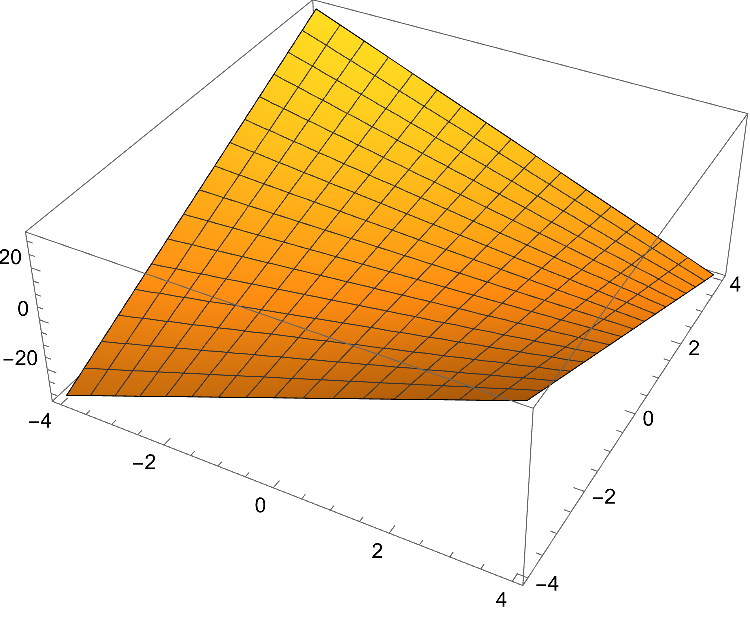
\includegraphics[width=\columnwidth]{source_compendium/figures/2503_18741/fig/harmonic_im.pdf}
        \caption{Imaginary part}
    \end{subfigure}
    \caption{Potential structure of harmonic oscillator, $-z^2$, in complex plane}
    \label{src:2503_18741:fig:V_harmonic}
\end{figure}
\begin{figure}
    \centering
    \begin{subfigure}{0.48\columnwidth}
        \centering
        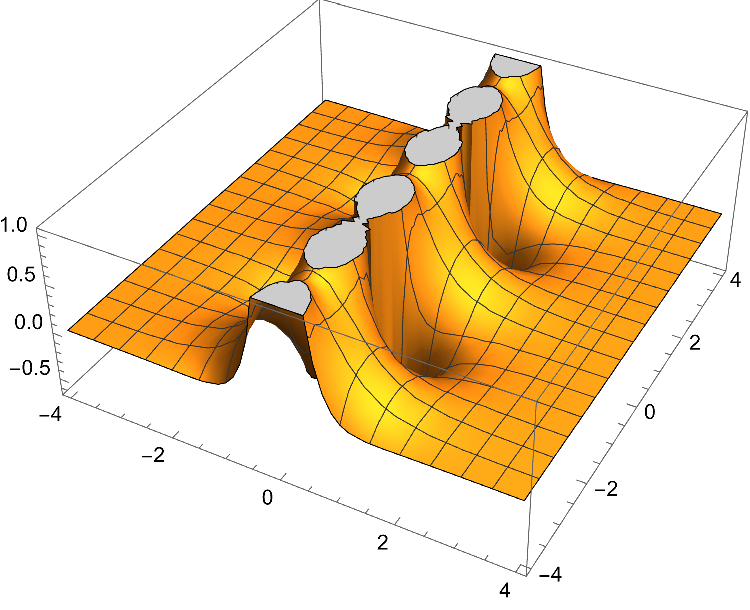
\includegraphics[width=\columnwidth]{source_compendium/figures/2503_18741/fig/cosh_re.pdf}
        \caption{Real part}
    \end{subfigure}\hspace*{1em}
    \begin{subfigure}{0.48\columnwidth}
        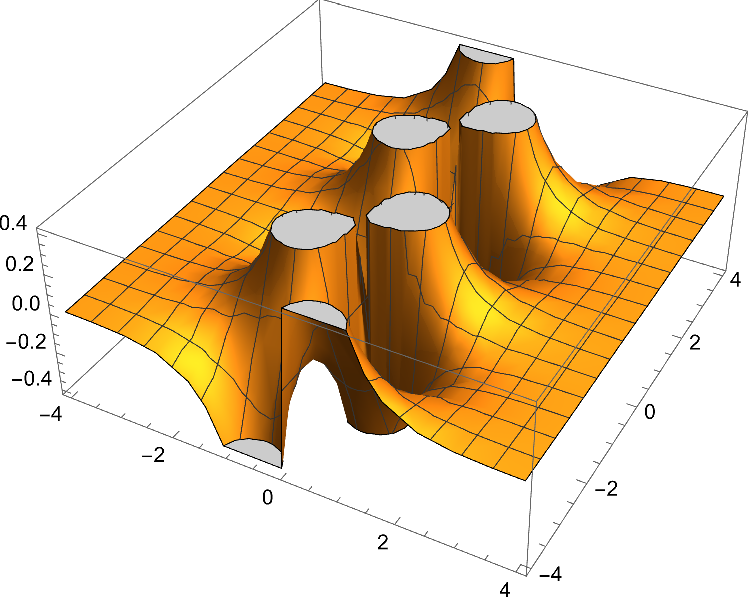
\includegraphics[width=\columnwidth]{source_compendium/figures/2503_18741/fig/cosh_im.pdf}
        \caption{Imaginary part}
    \end{subfigure}
    \caption{Potential structure of $1/\cosh^2{z}$ in complex plane}
    \label{src:2503_18741:fig:V_cosh}
\end{figure}
In what follows, we focus on an exactly solvable model, where we can see barrier resonant states explicitly.
Also, from the above picture, we will have the same complex energies by using the exact WKB analysis.
\subsubsection{Inverted Rosen--Morse potential}\label{src:2503_18741:sec:rm}
\paragraph{Exact solution}
Let us consider the inverted Rosen--Morse potential defined by
\begin{align}
    \left[-\frac{\hbar^2}{2m} \frac{\rmd^2}{\rmd x^2} + \frac{U_{0}}{\cosh^2 \beta x}\right] \psi(x)
    = E \psi(x) ,
    \qquad U_{0}>0.
\end{align}
This Schr\"odinger equation is exactly solvable as follows:
By using $\xi = \tanh \beta x$ and
\begin{align}
    k = \frac{\sqrt{2mE}}{\hbar}, \quad
    -\frac{2mU_{0}}{\beta^2\hbar^2} = s(s+1), \quad
    s=\frac{1}{2}\left( -1+\sqrt{1-\frac{8mU_{0}}{\beta^2 \hbar^2}} \right)
\end{align}
the equation can be rewritten as
\begin{align}
    \frac{\rmd}{\rmd \xi}\left[ (1-\xi^2) \frac{\rmd \psi}{\rmd \xi} \right] +
    \left[ s(s+1) - \left(\frac{\rmi k}{\beta}\right)^{2} \frac{1}{1-\xi^2} \right]\psi = 0 .
\end{align}
This is a general Legendre equation.
After changing variables as
\begin{align}
    \psi(x) = (1-\xi^2)^{\frac{\rmi k}{2\beta}} w(\xi)
\end{align} 
and $\frac{1}{2}(1-\xi)=u$, one finds the hypergeometric differential equation,
\begin{align}
    u(1-u)\frac{\rmd^2}{\rmd u^2}w + \left( \frac{\rmi k}{\beta} + 1 \right)(1-2u)\frac{\rmd}{\rmd u}w
    - \left( \frac{\rmi k}{\beta} - s \right) \left( \frac{\rmi k}{\beta} + s + 1 \right)w = 0 .
\end{align}
It is known that there are two independent solutions to the above equation.
One solution is finite at $\xi=1$, i.e. $x=\infty$, while another one is divergent there.
The former is given by
\begin{align}
    \psi(x) = 
    (1-\xi^2)^{-\frac{\rmi k}{2\beta}}
    F\left( -\frac{\rmi k}{\beta}-s, -\frac{\rmi k}{\beta}+s+1, -\frac{\rmi k}{\beta}+1, \frac{1-\xi}{2} \right) ,
 \label{src:2503_18741:eq:rm_sol}
\end{align}
where $F$ is the Gaussian hypergeometric function.
\paragraph{Traditional approach to resonance}\label{src:2503_18741:sec:rm_resonance}
The exact solution~\eqref{src:2503_18741:eq:rm_sol} has complex energies.
To see this from the traditional viewpoint,
the asymptotic behavior of the solution is of importance.
At first, in the case that $x\to\infty$, we see
\begin{align}
    (1-\xi^2)^{-\frac{\rmi k}{2\beta}}
% &=
% (1+\xi)^{-\frac{\rmi k}{2\beta}} (1-\xi)^{-\frac{\rmi k}{2\beta}}
% \notag \\
% &=
% (1+\xi)^{-\frac{\rmi k}{2\beta}}
% \left(
% 1-\frac{1-\rme^{-2 \beta x}}{1+\rme^{-2 \beta x}}
% \right)^{-\frac{\rmi k}{2\beta}}
% \notag \\
    &\to 
    4^{-\frac{\rmi k}{2\beta}} \rme^{\rmi kx}, 
\end{align}
and
\begin{align}
    F\left( -\frac{\rmi k}{\beta}-s, -\frac{\rmi k}{\beta}+s+1, -\frac{\rmi k}{\beta}+1, \frac{1-\xi}{2} \right)  
    \to 1 .
\end{align}
Thus, we have the asymptotic form of the exact solution at~$x\to\infty$
\begin{align}
    \psi(x) \rightarrow  4^{-\frac{\rmi k}{2\beta}} \rme^{\rmi kx} .
\end{align}
Here, the above expression means the transmitted wave.
Next, if $x\to-\infty$, the overall factor becomes
\begin{align}
    (1-\xi^2)^{-\frac{\rmi k}{2\beta}}
% &=
% (1+\xi)^{-\frac{\rmi k}{2\beta}} (1-\xi)^{-\frac{\rmi k}{2\beta}}
% \notag \\
% &=
% \left(
% 1-\frac{1-\rme^{2 \beta x}}{1+\rme^{2 \beta x}}
% \right)^{-\frac{\rmi k}{2\beta}}
% (1-\xi)^{-\frac{\rmi k}{2\beta}}
% \notag \\
    &\to
    (-4)^{-\frac{\rmi k}{2\beta}} \rme^{-\rmi kx} .
\end{align}
On the other hand, noting that
\begin{align}
    &F\left( -\frac{\rmi k}{\beta}-s, -\frac{\rmi k}{\beta}+s+1, -\frac{\rmi k}{\beta}+1, \frac{1-\xi}{2} \right) 
    \notag \\
    &=
    \frac{\Gamma\left(1-\frac{\rmi k}{\beta}\right) \Gamma\left(\frac{\rmi k}{\beta}\right)}{\Gamma(1+s) \Gamma(-s)}
    F\left( -\frac{\rmi k}{\beta}-s, -\frac{\rmi k}{\beta}+s+1, -\frac{\rmi k}{\beta}+1, \frac{1+\xi}{2} \right) 
    \notag \\
    &\qquad +
    \frac{\Gamma\left(1-\frac{\rmi k}{\beta}\right) \Gamma\left(-\frac{\rmi k}{\beta}\right)}
    {\Gamma\left(-\frac{\rmi k}{\beta}-s\right) \Gamma\left(-\frac{\rmi k}{\beta}+s+1\right)}
    \left(\frac{1+\xi}{2}\right)^{\frac{\rmi k}{a}}
    F\left( 1+s, -s, 1+\frac{\rmi k}{\beta}, \frac{1+\xi}{2} \right) 
\end{align}
the hypergeometric function behaves as
\begin{align}
    &F\left( -\frac{\rmi k}{\beta}-s, -\frac{\rmi k}{\beta}+s+1, -\frac{\rmi k}{\beta}+1, \frac{1-\xi}{2} \right) \notag\\
    &\to
    \frac{\Gamma\left(1-\frac{\rmi k}{\beta}\right) \Gamma\left(\frac{\rmi k}{\beta}\right)}{\Gamma(1+s) \Gamma(-s)}
    +
    \frac{\Gamma\left(1-\frac{\rmi k}{\beta}\right) \Gamma\left(-\frac{\rmi k}{\beta}\right)}
    {\Gamma\left(-\frac{\rmi k}{\beta}-s\right) \Gamma\left(-\frac{\rmi k}{\beta}+s+1\right)}
    \rme^{2\rmi kx} .
\end{align}
Therefore, we have in the $x\to-\infty$ region
\begin{align}
    \psi(x) &\to
    (-4)^{-\frac{\rmi k}{2\beta}} \rme^{-\rmi kx} 
    \frac{\Gamma\left(1-\frac{\rmi k}{\beta}\right) \Gamma\left(\frac{\rmi k}{\beta}\right)}{\Gamma(1+s) \Gamma(-s)} \notag\\&\qquad
    +
    (-4)^{-\frac{\rmi k}{2\beta}} \rme^{\rmi kx} 
    \frac{\Gamma\left(1-\frac{\rmi k}{\beta}\right) \Gamma\left(-\frac{\rmi k}{\beta}\right)}
    {\Gamma\left(-\frac{\rmi k}{\beta}-s\right) \Gamma\left(-\frac{\rmi k}{\beta}+s+1\right)},
\end{align}
where the first term on the right-hand side indicates the reflected wave, and the second term is the incident wave.
Imposing purely outgoing boundary conditions (Siegert boundary condition~\cite{Siegert:1939}) yields the resonance condition, where the coefficient of the incident wave~$\rme^{\rmi kx}$ vanishes.
%From the Siegert boundary condition~\cite{Siegert:1939}, the resonant solution is given in the case that the incident wave vanishes.
Hence, $\Gamma\left(-\frac{\rmi k}{\beta}-s\right)$ or $\Gamma\left(-\frac{\rmi k}{\beta}+s+1\right)$ should be divergent, and hence those Gamma functions become $\Gamma(-n)$ with a nonnegative integer $n$ (i.e. $n=0$, $1$, $2$, \dots). Therefore, this leads to discrete complex energies as follows:
%
\begin{itemize}
 \item The case that $\Gamma\left(-\frac{\rmi k}{\beta}+s+1\right)$ diverges.\\
  The divergence point of the Gamma function is expressed as
  \begin{align}
    -\frac{\rmi k}{\beta}+s+1=-n, \qquad \text{$n=0$, $1$, $2$, \dots} .
  \end{align}
  Solving this equation for $k$, we obtain
  \begin{align}
    k=\frac{\beta}{2}
    \left[-\rmi \sqrt{\frac{8mU_{0}}{\beta^2 \hbar^2}-1}-\rmi (2n+1)\right] .
  \end{align}
  Here, if the inequality, $1<8mU_{0}/(\beta^2 \hbar^2)$, is satisfied, the complex wave number and the complex energy are given by 
  \begin{align}
  \label{src:2503_18741:eq:wn-Res}
    \vsup{k}{R}_{n}=\frac{\beta}{2}
    \left[\sqrt{\frac{8mU_{0}}{\beta^2 \hbar^2}-1}-\rmi (2n+1)\right] 
  \end{align}
  and
  \begin{align}
    \vsup{E}{R}_{n}=\frac{\hbar^2 \beta^2}{8m}
    \left[\sqrt{\frac{8mU_{0}}{\beta^2 \hbar^2}-1}-\rmi (2n+1)\right]^2,
  \end{align}
  respectively. The wave number is in the fourth quadrant of the complex $k$-plane. Therefore, this solution corresponds to a resonant state.  \\
 \item The case that $\Gamma\left(-\frac{\rmi k}{\beta}-s\right)$ diverges.\\
  In the same way as the above case, we can obtain the divergence point of the Gamma function as
  \begin{align}
    -\frac{\rmi k}{\beta}-s=-n, \qquad \text{$n=0$, $1$, $2$, \dots},
  \end{align}
  which gives 
  \begin{align}
   \label{src:2503_18741:eq:wn-ARes}
    \vsup{k}{AR}_{n}=\frac{\beta}{2}
    \left[-\sqrt{\frac{8mU_{0}}{\beta^2 \hbar^2}-1}-\rmi (2n+1)\right]
  \end{align}
  and 
  \begin{align}
    \vsup{E}{AR}_{n}=\frac{\hbar^2 \beta^2}{8m}
    \left[\sqrt{\frac{8mU_{0}}{\beta^2 \hbar^2}-1}+\rmi (2n+1)\right]^2 .
  \end{align}
  The wave number is in the third quadrant of the complex $k$-plane. Equations \eqref{src:2503_18741:eq:wn-Res} and \eqref{src:2503_18741:eq:wn-ARes} satisfy the following relation:
  \begin{align}
    \vsup{k}{R}_{n} = - (\vsup{k}{AR}_{n})^{*},
  \end{align}
  which means that the state with $\vsup{k}{AR}_{n}$ is a time-reversal state of the resonant state, the so-called ``antiresonant state.''
\end{itemize}
\paragraph{Stokes graph}\label{src:2503_18741:sec:rm_stokes}
So far, we have derived the exact resonant solution and its energy.
Here, we proceed with the perspective of the exact WKB analysis.
Figure~\ref{src:2503_18741:fig:stokes_graph} shows the Stokes graph for the inverted Rosen--Morse potential, $V(x)=1/\cosh^2x$, with $0<E<1$.
The left and right panels are devoted to~$\im\hbar>0$ and $\im\hbar<0$, respectively.
The black points denote the turning points and the solid/dashed curves are the corresponding Stokes curves.
Note that the potential possesses the periodicity of~$\im x\in[-\pi/2,\pi/2]$ due to the cosine function on~$\re x=0$.
The blue point is the double pole and the blue wavy lines are branch cuts.
\begin{figure}[t]
\centering
\begin{tikzpicture}[scale=1]
  \draw[->] (-2.5,-1.4) -- (2.5,-1.4) node[right] {$\re x$};
  \draw[->] (0,-3) -- (0,3) node[above] {$\im x$};
  %
  \draw[thick,domain=0:520,samples=100,variable=\t,rotate=20] plot ({-0.002*\t*sin(\t)}, {-0.0018*\t^1.05*cos(\t)}) ..controls (0.5,1.35) and (1,1.1).. (1.4,1) node[above left] {$-$};
  \draw[thick,domain=0:-520,samples=100,variable=\t,rotate=20] plot ({0.002*\t*sin(\t)}, {-0.0018*\t^1.05*cos(\t)}) ..controls (-0.5,-1.35) and (-1,-1.1).. (-1.4,-1) node[below right] {$+$};
  \draw[thick,domain=0:550,samples=100,variable=\t,rotate=110] plot ({-0.0018*\t^1.05*sin(\t)}, {-0.002*\t*cos(\t)}) ..controls (1.5,0.9) and (1.5,0.4).. (1.7,0.5) node[below left] {$+$};
  \draw[thick,domain=0:-550,samples=100,variable=\t,rotate=110] plot ({0.0018*\t^1.05*sin(\t)}, {-0.002*\t*cos(\t)}) ..controls (-1.5,-0.9) and (-1.5,-0.4).. (-1.7,-0.5) node[above right] {$-$};
  %
  \draw[dashed] (1,1.4) ..controls (1.15,1.5) and (1.2,2) .. (0.9,2.8);
  \draw[dashed] (-1,-1.4) ..controls (-1.15,-1.5) and (-1.2,-2) .. (-0.9,-2.8);
  \draw[dashed] (-1,1.4)   ..controls (-0.5,1.4)   and (-0.2,1.6)  .. (0,1.7);
  \draw[dashed] (1,-1.4) ..controls (0.5,-1.4) and (0.2,-1.6) .. (0,-1.7);
  %
  \draw[thick] (1,1.4) ..controls (1.5,1) and (1.6,-1.4) .. (1.5,-2.8) node[right] {$+$};
  \draw[thick] (-1,-1.4) ..controls (-1.5,-1) and (-1.6,1.4) .. (-1.5,2.8) node[left] {$-$};
  %
  \fill[blue] (0,0) circle(4pt);
  \draw[very thick,blue, snake it] (-1,1.4) -- (1,-1.4);
  %
  \fill (-1,1.4) circle(3pt); \fill (1,1.4) circle(3pt);
  \fill (1,-1.4) circle(3pt); \fill (-1,-1.4) circle(3pt);
\end{tikzpicture}
\hspace{1em}
\begin{tikzpicture}[scale=1]
  \draw[->] (-2.5,-1.4) -- (2.5,-1.4) node[right] {$\re x$};
  \draw[->] (0,-3) -- (0,3) node[above] {$\im x$};
  %
  \fill (-1,1.4) circle(3pt); \fill (1,1.4) circle(3pt);
  \fill (1,-1.4) circle(3pt); \fill (-1,-1.4) circle(3pt);
  %
  \draw[thick,domain=0:-520,samples=100,variable=\t,rotate=-20] plot ({0.002*\t*sin(\t)}, {0.0018*\t^1.05*cos(\t)}) ..controls (-0.5,1.35) and (-1,1.1).. (-1.4,1) node[above right] {$+$};
  \draw[thick,domain=0:520,samples=100,variable=\t,rotate=-20] plot ({-0.002*\t*sin(\t)}, {0.0018*\t^1.05*cos(\t)}) ..controls (0.5,-1.35) and (1,-1.1).. (1.4,-1) node[below left] {$-$};
  \draw[thick,domain=0:-550,samples=100,variable=\t,rotate=-110] plot ({0.0018*\t^1.05*sin(\t)}, {0.002*\t*cos(\t)}) ..controls (-1.5,0.9) and (-1.5,0.4).. (-1.7,0.5) node[below right] {$-$};
  \draw[thick,domain=0:550,samples=100,variable=\t,rotate=-110] plot ({-0.0018*\t^1.05*sin(\t)}, {0.002*\t*cos(\t)}) ..controls (1.5,-0.9) and (1.5,-0.4).. (1.7,-0.5) node[above left] {$+$};
  %
  \draw[dashed] (-1,1.4) ..controls (-1.15,1.5) and (-1.2,2) .. (-0.9,2.8);
  \draw[dashed] (1,-1.4) ..controls (1.15,-1.5) and (1.2,-2) .. (0.9,-2.8);
  \draw[dashed] (1,1.4)   ..controls (0.5,1.4)   and (0.2,1.6)   .. (0,1.7);
  \draw[dashed] (-1,-1.4) ..controls (-0.5,-1.4) and (-0.2,-1.6) .. (0,-1.7);
  %
  \draw[thick] (-1,1.4) ..controls (-1.5,1) and (-1.6,-1.4) .. (-1.5,-2.8) node[left] {$-$};
  \draw[thick] (1,-1.4) ..controls (1.5,-1) and (1.6,1.4) .. (1.5,2.8) node[right] {$+$};
  %
  \fill[blue] (0,0) circle(4pt);
  \draw[very thick,blue, snake it] (1,1.4) -- (-1,-1.4);
\end{tikzpicture}
\caption{Schematically illustrated Stokes graph for the inverted Rosen--Morse potential, $V(x)=1/\cosh^2x$.
\textbf{(Left)} $\im\hbar>0$, \textbf{(right)} $\im\hbar<0$.
The black points denote the turning points and the solid curves are the corresponding Stokes curves.
The dashed ones, also Stokes curves, mean the periodicity of~$\im x\in[-\pi/2,\pi/2]$ due to the cosine function on~$\re x=0$.
The blue point is the double pole and the blue wavy lines are branch cuts.}
\label{src:2503_18741:fig:stokes_graph}
\end{figure}
To see the resonant states, we choose a path of the analytic continuation from~$\im x\to\pm\infty$ to~$\im x\to\mp\infty$ along the Stokes curves depicted in~Fig.~\ref{src:2503_18741:fig:stokes_graph}.
Especially, because of normalizability,
we need to take $\psi_-$ for both regions of~$\im x\to\pm\infty$.
Such a path can be chosen as shown in Fig.~\ref{src:2503_18741:fig:stokes_graph_path}.
The red path in the figure implies the path in the above sense.
%On the right panel, the monodromy coefficient should vanish.
Note that the red solid curve is on the Riemann sheet depicted
while the red dashed curve is on another Riemann sheet after passing through the branch cut.
\begin{figure}[t]
\centering
\begin{tikzpicture}[scale=1.4]
  \draw[->] (-2.5,-1.4) -- (2,-1.4) node[right] {$\re x$};
  \draw[->] (0,-3.3) -- (0,1.1) node[above] {$\im x$};
  %
  \draw[thick,rotate around={20:(0,-1.4)}] (1,-1.4) ..controls (1.15,-1.3) and (1.2,-0.8) .. (0.9,0) node[above] {$-$};
  \draw[thick,rotate around={20:(0,-1.4)}] (-1,-1.4) ..controls (-1.15,-1.5) and (-1.2,-2) .. (-0.9,-2.8) node[left] {$+$};
  \draw[thick,rotate around={20:(0,-1.4)}] (-1,-1.4)   ..controls (-0.5,-1.4)   and (0,-1.2)  .. (0.6,-0.5) node[midway,above left] {$+$};
  \draw[thick,rotate around={20:(0,-1.4)}] (1,-1.4) ..controls (0.5,-1.4) and (0,-1.6) .. (-0.6,-2.3) node[midway,below right] {$-$};
  %
  \draw[thick,rotate around={20:(0,-1.4)}] (1.2,0.5) ..controls (1.4,0) and (1.6,-1.4) .. (1.5,-2.8) node[right] {$+$};
  \draw[thick,rotate around={20:(0,-1.4)}] (-1,-1.4) ..controls (-1.5,-1) and (-1.6,1) .. (-1.6,1) node[left] {$-$};
  \draw[thick,rotate around={20:(0,-1.4)}] (1,-1.4) ..controls (1.4,-1.6) and (1.3,-2.5) .. (1.3,-2.8) node[left] {$+$};
  %
  \draw[ultra thick,red,rotate around={20:(0,-1.4)}] (-1.4,1) ..controls (-1.3,0) and (-1.3,-0.5) .. (-1,-1.1) -- (0.76,-1.1);
  \draw[ultra thick,dotted,red,->,rotate around={20:(0,-1.4)}] (0.76,-1.1) -- (1.3,-1.1) .. controls (1.4,-1.8) and (1.4,-2.4) .. (1.4,-2.8);
  %
  \fill[blue] (0,0) circle(3pt); \fill[blue] (0,-2.8) circle(3pt);
  \draw[blue, snake it,rotate around={20:(0,-1.4)}] (0.43,0.01) -- (1,-1.4);
  \draw[blue, snake it,rotate around={20:(0,-1.4)}] (-0.43,-2.81) -- (-1,-1.4);
  %
  \fill[rotate around={20:(0,-1.4)}] (1,-1.4) circle(3pt); \fill[rotate around={20:(0,-1.4)}] (-1,-1.4) circle(3pt);
  %
  \draw[very thick,dashed,teal,rotate around={20:(0,-1.4)}] (0,-1.4) circle [x radius=1.3,y radius=0.4] node[below left] {$A$};
\end{tikzpicture}
%\hspace{1em}
%\begin{tikzpicture}[scale=1.4]
%  \draw[->] (-2.5,-1.4) -- (2,-1.4) node[right] {$\re x$};
%  \draw[->] (0,-3.3) -- (0,1.1) node[above] {$\im x$};
%  %
%  \draw[thick,rotate around={20:(0,-1.4)}] (1,-1.4) ..controls (1.15,-1.3) and (1.2,-0.8) .. (0.9,0) node[above] {$-$};
%  \draw[thick,rotate around={20:(0,-1.4)}] (-1,-1.4) ..controls (-1.15,-1.5) and (-1.2,-2) .. (-0.9,-2.8) node[left] {$+$};
%  \draw[thick,rotate around={20:(0,-1.4)}] (-1,-1.4)   ..controls (-0.5,-1.4)   and (0,-1.2)  .. (0.6,-0.5) node[midway,above left] {$+$};
%  \draw[thick,rotate around={20:(0,-1.4)}] (1,-1.4) ..controls (0.5,-1.4) and (0,-1.6) .. (-0.6,-2.3) node[midway,below right] {$-$};
%  %
%  \draw[thick,rotate around={20:(0,-1.4)}] (1.2,0.5) ..controls (1.4,0) and (1.6,-1.4) .. (1.5,-2.8) node[right] {$+$};
%  \draw[thick,rotate around={20:(0,-1.4)}] (-1,-1.4) ..controls (-1.5,-1) and (-1.6,1) .. (-1.6,1) node[left] {$-$};
%  \draw[thick,rotate around={20:(0,-1.4)}] (1,-1.4) ..controls (1.4,-1.6) and (1.3,-2.5) .. (1.3,-2.8) node[left] {$+$};
%  %
%  \draw[ultra thick,red,rotate around={20:(0,-1.4)}] (-1.4,1) ..controls (-1.3,0) and (-1.3,-0.5) .. (-1,-1.1) -- (0.76,-1.1);
%  \draw[ultra thick,red,->,rotate around={20:(0,-1.4)}] (0.76,-1.1) -- (1.3,-1.1) .. controls (1.4,-1.8) and (1.4,-2.4) .. (1.4,-2.8);
%  %
%  \fill[blue] (0,0) circle(3pt); \fill[blue] (0,-2.8) circle(3pt);
%  \draw[blue, snake it,rotate around={20:(0,-1.4)}] (0.43,0.01) -- (1,-1.4);
%  \draw[blue, snake it,rotate around={20:(0,-1.4)}] (-0.43,-2.81) -- (-1,-1.4);
%  %
%  \fill[rotate around={20:(0,-1.4)}] (1,-1.4) circle(3pt); \fill[rotate around={20:(0,-1.4)}] (-1,-1.4) circle(3pt);
%  %
%  \draw[very thick,dashed,teal,rotate around={20:(0,-1.4)}] (0,-1.4) circle [x radius=1.3,y radius=0.4] node[below left] {$A$};
%\end{tikzpicture}
\caption{Quantization condition with~$\im\hbar>0$ and~$\im E<0$.
The red path is an option to carry out the analytical continuation,
along which we can normalize the exact WKB solution.
%on the left panel but cannot have any solution on the right panel.
The nontrivial cycle, $A$-cycle, is shown as the green dashed loop.}
\label{src:2503_18741:fig:stokes_graph_path}
\end{figure}
We make a remark on analogy to the CSM. From the ABC theorem, resonant states after complex scaling are some kind of bound states. It indicates that resonant states can be normalized in complexified asymptotic regions. In fact, in the Stokes graph in Fig.~\ref{src:2503_18741:fig:stokes_graph_path}, we observe that there is a path in the complex plane along which the wave function decays; we regard it as the normalizable path.
Figure~\ref{src:2503_18741:fig:stokes_graph_path} gives rise to the following quantization condition
along the red arrowed path:
% on the left panel
\begin{align}
    1 - A = 0 .
    \label{src:2503_18741:eq:quantization_cond}
\end{align}
%while that on the right panel is
%\begin{align}
%    1 + A = 0.
%    \label{src:2503_18741:eq:quantization_cond_anti}
%\end{align}
(A more rigorous derivation under regularization is provided in Sec.~\ref{lab:2505_02301}.)
Here, $A$ is the nontrivial cycle, the $A$-cycle, shown as the green dashed loop.
From now on, let us calculate $A$
in the leading order of the exact WKB
and a completely exact analysis.
\paragraph{Leading order}\label{src:2503_18741:sec:rm_leading}
In the leading order,
we carry out an integral of the WKB approximation between the turning points:
\begin{align}
    \int_{-\cosh^{-1}\sqrt{\frac{1}{E}}}^{\cosh^{-1}\sqrt{\frac{1}{E}}} \rmd x \sqrt{2(V(x) - E)}
    = \sqrt{2} \int \rmd x\sqrt{\frac{1}{\cosh^2 x} - E} .
\end{align}
Here we set almost all parameters as units for simplicity.
After some calculations, we find that
\begin{align}
    &\int_{-\cosh^{-1}\sqrt{\frac{1}{E}}}^{\cosh^{-1}\sqrt{\frac{1}{E}}} \rmd x \sqrt{2(V(x) - E)}\notag\\
%    &= -\frac{1}{E \cosh (2x)+E-2}
%   \Biggl\{
%   2 \cosh (x)
%   \sqrt{-E-\tanh ^2(x)+1}
%   \notag\\&\qquad\times
%   \Biggl(
%   \sqrt{E \cosh (2 x)+E-2} \tanh^{-1} \left(\frac{\sqrt{2} \sinh (x)}{\sqrt{E \cosh (2 x)+E-2}}\right)
%   \notag\\&\qquad\qquad
%   -\sqrt{E-1} \sqrt{E} \sinh ^{-1}\left(\frac{\sinh(x)}{\sqrt{1-\frac{1}{E}}}\right) \sqrt{\frac{E \cosh (2 x)+E-2}{E-1}}
%   \Biggr)
%   \Biggr\}
%   \\
    &= - 2 \cosh (x) 
   \sqrt{\frac{-E-\tanh ^2(x)+1}{E \cosh (2 x)+E-2}}
   \notag\\&\qquad\times
   \left[
   \tanh^{-1} \left(\frac{\sqrt{2} \sinh (x)}{\sqrt{E \cosh (2 x)+E-2}}\right)
   -\sqrt{E} \sinh ^{-1}\left(\frac{\sinh(x)}{\sqrt{1-\frac{1}{E}}}\right)
   \right]
   \\
    &= \mp \sqrt{2}\,\rmi
   \left[
   \tanh^{-1} \left(\frac{\sqrt{2} \sinh (x)}{\sqrt{E \cosh (2 x)+E-2}}\right)
   -\sqrt{E} \sinh ^{-1}\left(\frac{\sinh(x)}{\sqrt{1-\frac{1}{E}}}\right)
   \right]
   \\
   &= \pm \sqrt{2} \pi (1 + \sqrt{E}) .
\end{align}
Then, from the quantization condition~\eqref{src:2503_18741:eq:quantization_cond},
\begin{align}
    2 \sqrt{2} \pi (1 + \sqrt{E}) = 2\pi \rmi n,
\end{align}
with $n\in\mathbb{Z}$.
Therefore, the leading complex energy is given by
\begin{align}
    E = \left( 1 - \frac{\rmi n}{\sqrt{2}} \right)^2 .
\end{align}
%Also, we have another complex energy by replacing $n$ with $n+\frac{1}{2}$ for the other condition~\eqref{src:2503_18741:eq:quantization_cond_anti}.
This is quite suggestive because we observe resonance in the fourth quadrant even in the leading order of the exact WKB method.\footnote{For the usual (noninverted) Rosen--Morse potential, higher-order contribution from~$S_i$ vanishes. (This is the reason why it possesses shape invariance in the same way as the harmonic oscillator.) Then, one finds an exact solution. On the other hand, higher-order terms $S_i$ do not vanish for the inverted Rosen--Morse potential. We need some careful treatment.}
\paragraph{Exact WKB analysis for resonance}\label{src:2503_18741:rm_ewkb}
In the above Stokes graphs, the exact solution on the normalizable path
is explicitly written by the exact solution~\eqref{src:2503_18741:eq:rm_sol}.
Note that another solution has opposite signs for Stokes curves.
This means that the WKB solution can be exactly given by
\begin{align}
    \rme^{\int_{x_0}^{x} \rmd x' \vsub{S}{odd}}
    = \left.(1-\xi^2)^{-\frac{\rmi k}{2\beta}}
    F\left( -\frac{\rmi k}{\beta}-s, -\frac{\rmi k}{\beta}+s+1, -\frac{\rmi k}{\beta}+1, \frac{1-\xi}{2} \right)\right|_{\text{at $x$}},
\end{align}
where $x_0$ is a reference point.
The $A$-cycle, $\rme^{\oint \vsub{S}{odd}}$, between turning points
$\mp\cosh^{-1}\sqrt{U_0/E}$ can be realized by the exchange of reference points.
That is,
\begin{align}
    \rme^{2\int_{x_0}^{\cosh^{-1}\sqrt{U_0/E}} \rmd x\, \vsub{S}{odd}}
    \times \rme^{-2\int_{x_0}^{-\cosh^{-1}\sqrt{U_0/E}} \rmd x\, \vsub{S}{odd}}
    = \rme^{2\int_{-\cosh^{-1}\sqrt{U_0/E}}^{\cosh^{-1}\sqrt{U_0/E}} \rmd x\, \vsub{S}{odd}} .
\end{align}
From the fact that $A=1$ for the existence of a normalizable solution, we see
\begin{align}
    \left[
    \frac{F\left( -\frac{\rmi k}{\beta}-s, -\frac{\rmi k}{\beta}+s+1, -\frac{\rmi k}{\beta}+1, \frac{1-|\xi|}{2} \right)}
    {F\left( -\frac{\rmi k}{\beta}-s, -\frac{\rmi k}{\beta}+s+1, -\frac{\rmi k}{\beta}+1, \frac{1+|\xi|}{2} \right)}
    \right]^2
    = 1 ,
    \label{src:2503_18741:eq:quant_cond_F}
\end{align}
where $|\xi|=\tanh(\beta\cosh^{-1}\sqrt{U_0/E})$.
Here, we use the formula of the hypergeometric function as
\begin{align}
    &F\left( -\frac{\rmi k}{\beta}-s, -\frac{\rmi k}{\beta}+s+1, -\frac{\rmi k}{\beta}+1, \frac{1\pm|\xi|}{2} \right)\notag\\
    &= \mathfrak{A} F\left(-\frac{\rmi k}{2\beta}-\frac{s}{2},-\frac{\rmi k}{2\beta}+\frac{s+1}{2},\frac{1}{2},|\xi|^2\right)
    \notag\\
    &\quad\mp \mathfrak{B} F\left(-\frac{\rmi k}{2\beta}-\frac{s-1}{2},-\frac{\rmi k}{2\beta}+\frac{s}{2}+1,\frac{3}{2},|\xi|^2\right) \notag\\
    &\equiv \mathfrak{A} F_A \mp \mathfrak{B} F_B,
\end{align}
where
\begin{align}
    \mathfrak{A} &= \frac{\Gamma\left(-\frac{\rmi k}{\beta}+1\right)\Gamma\left(\frac{1}{2}\right)}
    {\Gamma\left(-\frac{\rmi k}{2\beta}-\frac{s-1}{2}\right)\Gamma\left(-\frac{\rmi k}{2\beta}+\frac{s}{2}+1\right)},
    \notag\\
    \mathfrak{B} &= \frac{\Gamma\left(-\frac{\rmi k}{\beta}+1\right)\Gamma\left(-\frac{1}{2}\right)}
    {\Gamma\left(-\frac{\rmi k}{2\beta}-\frac{s}{2}\right)\Gamma\left(-\frac{\rmi k}{2\beta}+\frac{s+1}{2}\right)} .
\end{align}
Substituting this into the quantization condition~\eqref{src:2503_18741:eq:quant_cond_F}, we find that
\begin{align}
    \left(\frac{\mathfrak{A} F_A + \mathfrak{B} F_B}{\mathfrak{A} F_A - \mathfrak{B} F_B}\right)^2 = 1 .
\end{align}
To obtain $(+1)^2$ on the left-hand side in Eq.~\eqref{src:2503_18741:eq:quant_cond_F}, it is easy to find $\mathfrak{B}=0$.
Therefore, $\Gamma\left(-\frac{\rmi k}{2\beta}-\frac{s}{2}\right)$ or
$\Gamma\left(-\frac{\rmi k}{2\beta}+\frac{s+1}{2}\right)$ should be at pole singularities.
Then, $-\frac{\rmi k}{\beta}-s=-2n$ or $-\frac{\rmi k}{\beta}+s+1=-2n$ ($n=0$, $1$, \dots).
The former corresponds to antiresonance and the latter is resonance,
being identical to the above observation in~Section~\ref{src:2503_18741:sec:rm_resonance} with \textit{even} numbers of nodes.
On the other hand, we also have another condition when the left-hand side in Eq.~\eqref{src:2503_18741:eq:quant_cond_F} becomes $(-1)^2$; then, $\Gamma\left(-\frac{\rmi k}{2\beta}-\frac{s-1}{2}\right)$ or $\Gamma\left(-\frac{\rmi k}{2\beta}+\frac{s}{2}+1\right)$ should diverge such that $\mathfrak{A}=0$.
Then, $-\frac{\rmi k}{\beta}-s=-2n-1$ or $-\frac{\rmi k}{\beta}+s+1=-2n-1$ ($n=0$, $1$, \dots).
This is a completely identical result to the complex energies with \textit{odd} numbers of nodes.
Totally, indeed, one finds that $-\frac{\rmi k}{\beta}-s=-n$ or $-\frac{\rmi k}{\beta}+s+1=-n$ ($n=0$, $1$, \dots), which is identical to~$\vsup{E_n}{AR}$ or $\vsup{E_n}{R}$, respectively.\footnote{In contrast to Gamow’s method which yields an exponentially small imaginary part for the energy from the leading tunneling action, the exact WKB method systematically incorporates all orders and treats the resonance condition with full analytical rigor (as in Eq.~\eqref{src:2503_18741:eq:quant_cond_F}).}

\subsection*{Laboratory checkpoint}
Before moving to the next stage, perform the following checks without copying
the displayed final answer.
\begin{enumerate}
  \item Recompute the ordered product of Stokes matrices and identify the entry that multiplies the prohibited incoming branch.
  \item Derive the resonance condition both from the exact hypergeometric solution and from the exact-WKB connection coefficient.
  \item Change the continuation path or lateral Borel side and record how the sheet label changes while the physical pole remains consistent.
\end{enumerate}
